\documentclass[12pt,twoside]{report}

\usepackage[utf8]{inputenc}
\usepackage[spanish]{babel}

\usepackage{amsmath}
\usepackage{amsfonts}
\usepackage{amssymb}

\usepackage{setspace}

\usepackage{enumitem}

\usepackage[normalem]{ulem}

\usepackage[table,xcdraw]{xcolor}

\usepackage[export]{adjustbox}
\usepackage[official]{eurosym}
\usepackage{longtable}

\usepackage{wrapfig}

%%%%%%%%%%%%%%%%%%%%%%%%%%%%%%%%%%%%%%%%%%%%%%%%%%%%%%%%%%%%%%%%%%%%%%%%%%%%%

% Definitions for the title page
\newcommand{\reporttitle}{
	Solicitud de Subvención\\
	y \\
	Memoria de Actividades 2014-15
}
\newcommand{\reportauthor}{Asociación Club de Robótica-Mecatrónica}



\setlength{\parskip}{\baselineskip}
\setlength{\parindent}{0pt}

\usepackage{hyperref}
\hypersetup{
    hyperindex, linktoc=page, breaklinks,
    pdfauthor=\reportauthor,pdftitle=\reporttitle
}
%%%%%%%%%%%%%%%%%%%%%%%%%%%%%%%%%%%%%%%%%%%%%%%%%%%%%%%%%%%%%%%%%%%%%%%%%%%%%

% load some definitions and default packages
%%%%%%%%%%%%%%%%%%%%%%%%%%%%%%%%%%%%%%%%%
% University Assignment Title Page 
% LaTeX Template
% Version 1.0 (27/12/12)
%
% This template has been downloaded from:
% http://www.LaTeXTemplates.com
%
% Original author:
% WikiBooks (http://en.wikibooks.org/wiki/LaTeX/Title_Creation)
%
% License:
% CC BY-NC-SA 3.0 (http://creativecommons.org/licenses/by-nc-sa/3.0/)
% 
%
%%%%%%%%%%%%%%%%%%%%%%%%%%%%%%%%%%%%%%%%%
%----------------------------------------------------------------------------------------
%	PACKAGES AND OTHER DOCUMENT CONFIGURATIONS
%----------------------------------------------------------------------------------------
%\usepackage[a4paper,left=2.8cm,right=2.8cm,vmargin=2.0cm,includeheadfoot]{geometry}
\usepackage[a4paper,left=3.5cm,right=2.1cm,vmargin=2.0cm,includeheadfoot]{geometry}

\usepackage{textpos}

\usepackage{tabularx,longtable,multirow,subfigure,caption}
\usepackage{fncylab} %formatting of labels
\usepackage{fancyhdr} % page layout
\usepackage{url} % URLs

\usepackage{amsmath}
\usepackage{graphicx}
\usepackage{dsfont}

\usepackage{array}
\usepackage{latexsym}



%%% Default fonts
\renewcommand*{\rmdefault}{bch}
\renewcommand*{\ttdefault}{cmtt}



%%% Default settings (page layout)
\setlength{\parindent}{0em}  % indentation of paragraph

\setlength{\headheight}{14.5pt}
\pagestyle{fancy}
\renewcommand{\chaptermark}[1]{\markboth{\chaptername\ \thechapter.\ #1}{}} 

\fancyfoot[EL,OR]{\sffamily\textbf{\thepage}}%Page no. in the left on odd pages and on right on even pages
\fancyfoot[OC,EC]{\sffamily }
\renewcommand{\headrulewidth}{0.1pt}
\renewcommand{\footrulewidth}{0.1pt}
\captionsetup{margin=10pt,font=small,labelfont=bf}


%--- chapter heading

\def\@makechapterhead#1{%
  \vspace*{10\p@}%
  {\parindent \z@ \raggedright \sffamily
    \interlinepenalty\@M
    \Huge\bfseries \thechapter \space\space #1\par\nobreak
    \vskip 30\p@
  }}

%---chapter heading for \chapter*  
\def\@makeschapterhead#1{%
  \vspace*{10\p@}%
  {\parindent \z@ \raggedright
    \sffamily
    \interlinepenalty\@M
    \Huge \bfseries  #1\par\nobreak
    \vskip 30\p@
  }}

\allowdisplaybreaks


\date{Diciembre de 2015}

\addto\captionsspanish{\renewcommand{\chaptername}{Parte}}

\begin{document}

\begin{titlepage}

\newcommand{\HRule}{\rule{\linewidth}{1mm}} % Defines a new command for the horizontal lines, change thickness here


%----------------------------------------------------------------------------------------
%	LOGO SECTION
%----------------------------------------------------------------------------------------


\includegraphics[width = 6cm]{fotos/logo-eps.png}
\hfill

\includegraphics[width = 6cm]{fotos/logo-uam.png}



\center % Center remainder of the page

%----------------------------------------------------------------------------------------
%	HEADING SECTIONS
%----------------------------------------------------------------------------------------

%\textsc{\Large Escuela Politécnica Superior}\\[0.1cm]
%\textsc{\Large Universidad Autónoma de Madrid}\\[0.5cm]
\vspace{1cm}

%----------------------------------------------------------------------------------------
%	TITLE SECTION
%----------------------------------------------------------------------------------------


\HRule \\[0.4cm]
\begin{spacing}{1.5}
{ \fontsize{0.8cm}{1em} \bfseries \reporttitle}\\ % Title of your document
\vspace{0.5cm}
{ \fontsize{0.7cm}{1em} \bfseries \reportauthor} \\
\end{spacing}
\HRule \\[1.5cm]



\includegraphics[width = 7cm]{fotos/logo_crm-192x192.png}

{\large Asociación Club de Robótica-Mecatrónica (CRM-UAM)} \\
Local B-111 -- Escuela Politécnica Superior

\vfill

\textsc{\Large Universidad Autónoma de Madrid}\\[0.5cm]

\vfill

%----------------------------------------------------------------------------------------
%	FOOTER & DATE SECTION
%----------------------------------------------------------------------------------------


\makeatletter
{ \Large \@date }
\vfill
\makeatother


\end{titlepage}

\clearpage{\pagestyle{empty}\cleardoublepage}


% page numbering etc.
\pagenumbering{roman}
\setcounter{page}{1}
\pagestyle{fancy}






\begin{spacing}{0.1}
\tableofcontents
\end{spacing}

\clearpage{\pagestyle{empty}\cleardoublepage}

\pagenumbering{arabic}
\setcounter{page}{1}

\fancyhead[LE,RO]{\slshape}
%\fancyhead[LE,RO]{\slshape \rightmark}
\fancyhead[LO,RE]{\slshape \leftmark}

%%%%%%%%%%%%%%%%%%%%%%%%%%%%%%%%%%%%


\chapter{Presupuesto para nuevas actividades}


\section{Renovación del taller del club de robótica}
\subsubsection{Introduccion}

\section{Proyectos de construcción propia}

\subsection{Adaptación del cuadricóptero para vuelo autónomo}
\subsubsection{Responsable de proyecto y equipo de trabajo}
Jaime y Rodrigo
\subsubsection{Descripción}
Tal y como se detalla en la memoria de actividades, el año pasado presentamos un presupuesto para la construcción de un drone.

Como recordatorio la idea principal era construir un cuadricóptero manejado por control remoto capaz de detectar y evitar obstáculos en un modo de control autónomo.

Durante el pasado año académico completamos con éxito la primera parte del proyecto y ya tenemos construido y calibrado el cuadricóptero que ha pasado satisfactoriamente las primeras pruebas de vuelo teleoperado.


\begin{figure}[hbtp]
\centerline{
    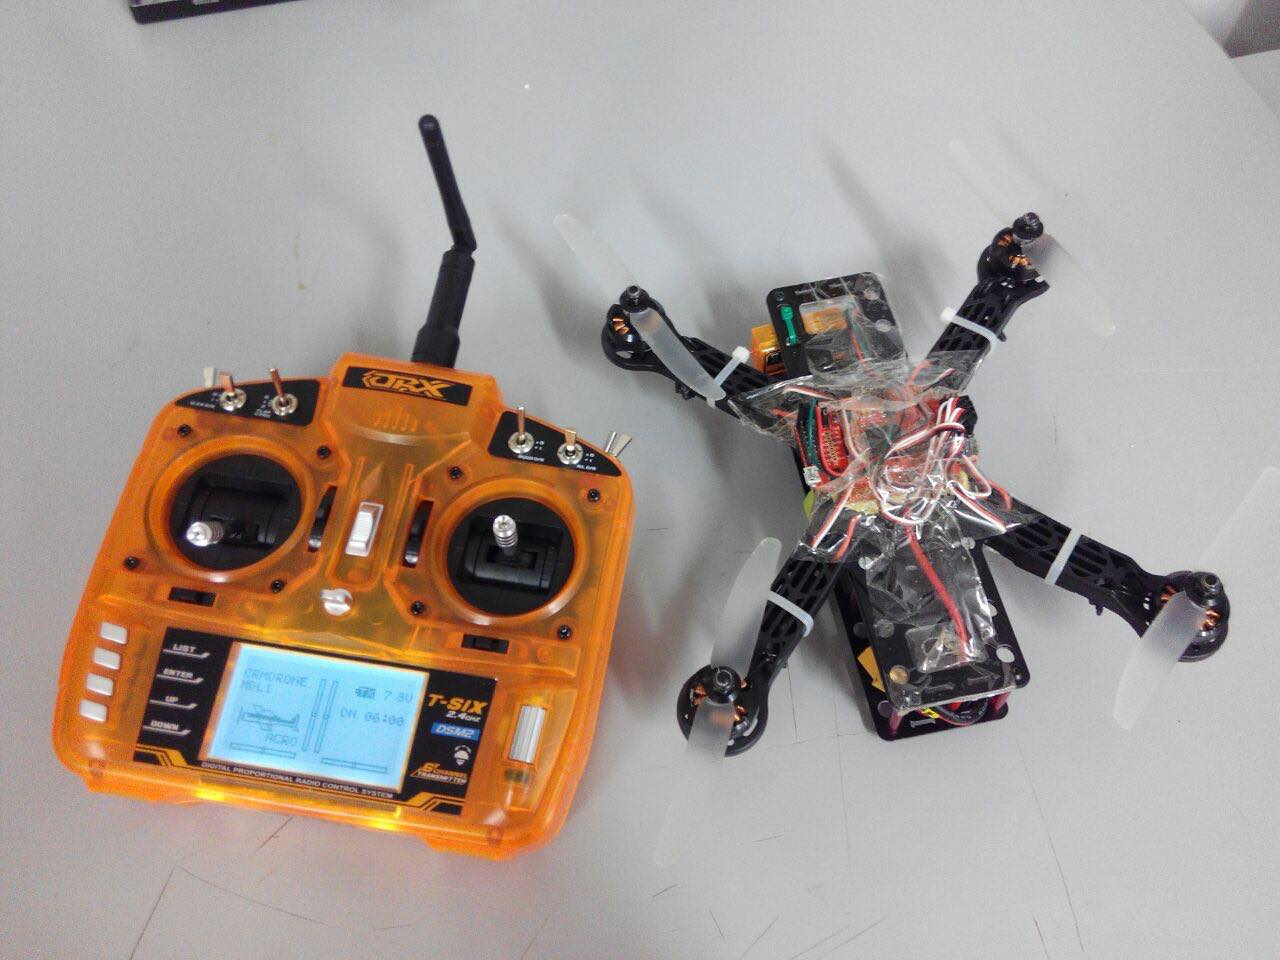
\includegraphics[width=0.45\linewidth]{fotos/dron1.jpg}
    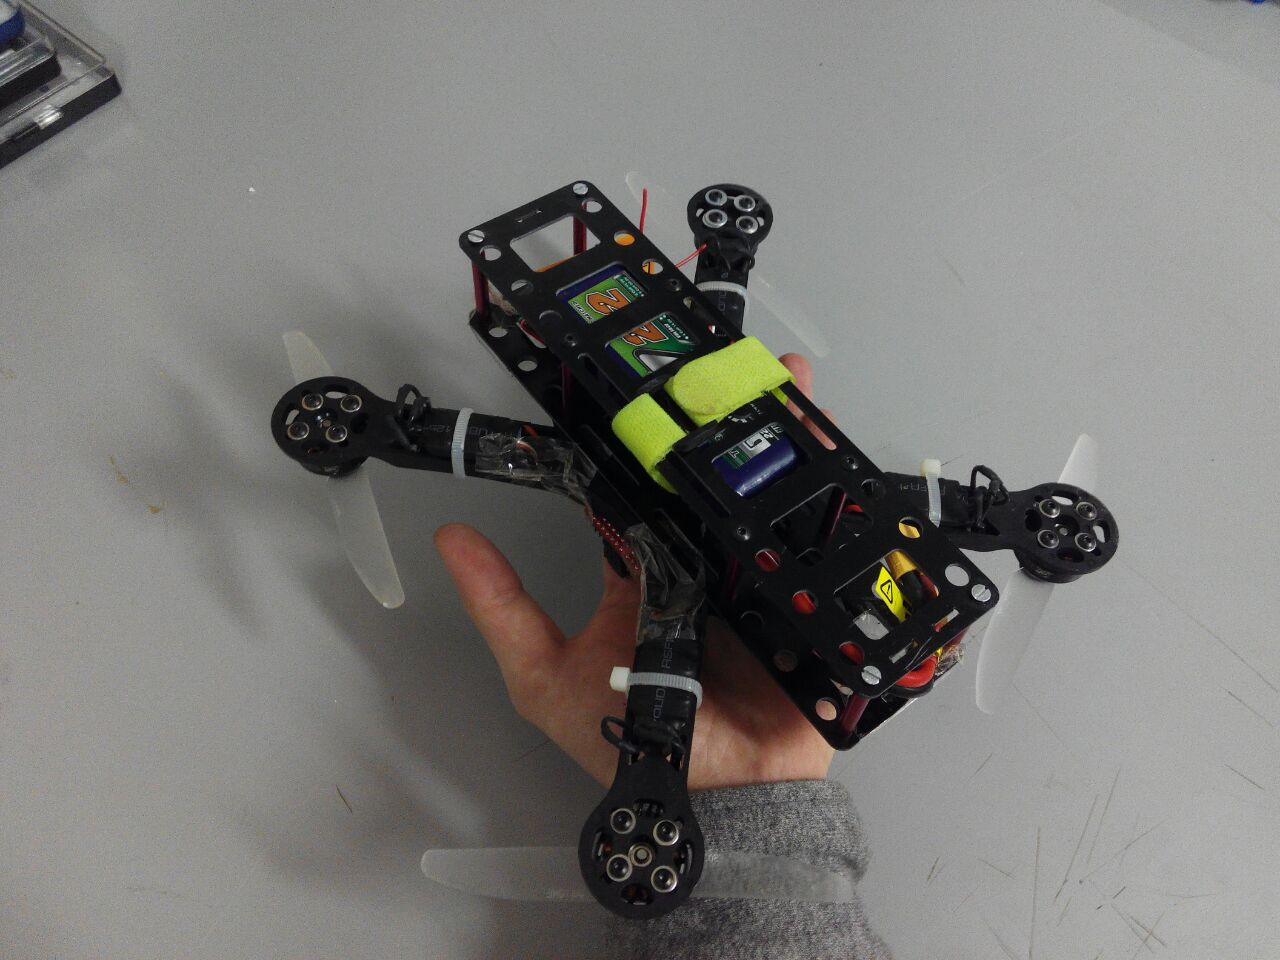
\includegraphics[width=0.45\linewidth]{fotos/dron2.jpg}}
\caption*{
Fotos del proceso de construcción del dron.}
\end{figure}

Queremos por tanto duante este próximo curso proseguir con el proyecto realizando el módulo de vuelo autónomo.

\subsubsection{Objetivos}

\subsubsection{Detalles y Contenido}
Nuestra intención es filtrar las señales que llegan al receptor del cuadricóptero mediante las medidas de los sensores ultrasónicos y con ayuda de la arduino para evitar posibles colisiones.

Existen numerosos cuadricóptero ya fabricados que disponen de GPS y son semi-autónomos puesto que se les proporcionan unas coordenadas y este realiza la ruta deseada, pero siempre en campo abierto y sin obstáculos.

Por eso queremos marcar la diferencia e intentar diseñar uno de los primeros cuadricópteros que no solo fuesen capaces de ir hasta unas determinadas coordenadas en campo abierto, sino que fuese capaz de detectar los obstáculos que se encuentre a su paso y los evite, modificando la ruta inicial gracias a los sensores y los cálculos realizados por la controladora.


\subsubsection{Previsión de desarrollo}
En la primera parte de este proyecto nos hemos dedicado exclusivamente a la fabricación de un Drone básico para lo cual hemos comprado las partes principales como son la estructura, motores, variadores, bateria, mando, receptor, y la controladora de vuelo (con GPS). Una vez concluida satisfactoriamente esta primera parte , es decir, habiendo construido el cuadricoptero y lograr pilotarlo, nos disponemos a pedir presupuesto para la continuación de este proyecto.

Al empezar este proyecto parecía algo ambicioso y difícil de llevar a cabo pero hemos construido un drone completamente funcional y lo hemos calibrado para que tenga unas condiciones de vuelo óptimas, por lo que vemos mucho más cerca el poder llevar a cabo la idea inicial y comenzar este año con la continuación de nuestro prototipo para que sea capaz de volar de manera autónoma o ser controlado de forma remota en primera persona (con unas gafas de realidad virtual FPV  first person view). Esta es nuestra meta debido a que sería lo que realmente diferenciaría nuestro trabajo en el CRM de otros proyectos, ya que la idea de que sea completamente autónomo es pionera en el campo y debido a la diversidad de estudiantes (Telecomunicación, informática y doble grado de informática y matemáticas) creemos que tenemos los conocimientos para llevarlo a cabo.

\subsubsection{Presupuesto}
El coste de las piezas se disparó debido a unos gastos de aduanas bastante más elevados de lo esperado.

Por lo que con el presupuesto de este año hemos podido construir únicamente el drone (sin elementos de visión artificial ni sensores necesarios para el vuelo autónomo) concluyendo así lo que podríamos denominar la primera parte del proyecto.

Enumeramos a continuación los elementos presupuestados para esta segunda fase, junto con su precio, enlace de compra y la descripción y justificación:

\begin{itemize}
\item  {\bf Sensor de distancia por ultrasonidos [x6] 18,03\euro{}/u}

Enlace: \url{www.electan.com/sensor-distancia-por-ultrasonidos-ping-p-3134.html}

Con estos sensores pretendemos detectar obstaculos en cualquiera de las seis direciones posibles de movimiento del dron (norte, sur, este, oeste, y los dos movimientos verticales) creando un mapa virtual de obtaculos y pudiendo así evitarlos modificando la ruta óptima lo menos posibles.

\centerline{
    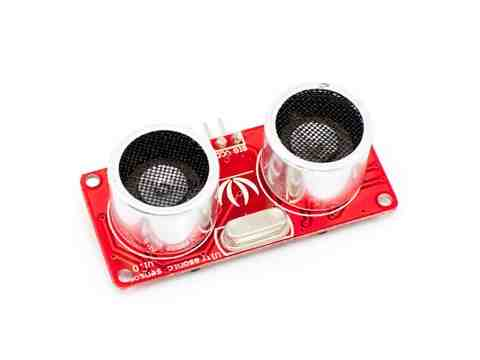
\includegraphics[width=0.45\linewidth]{fotos/sensor_ultra.jpg}}

\item {\bf Helices eficientes (HQ 6") [x3 packs] 5,30\euro{}.}

Enlace: \url{flyduino.net/Multikopter-Propeller-CW-CCW_44}

Sin duda las hélices  son las partes del drone que más expuestas a colisiones están. Por ello pedimos presupuesto para comprar 3 juegos de este tipo hélices, que además son de una calidad alta lo que disminuirá el riesgo a que se partan, pero aun así, es seguro, que necesitaremos recambios.

\centerline{
    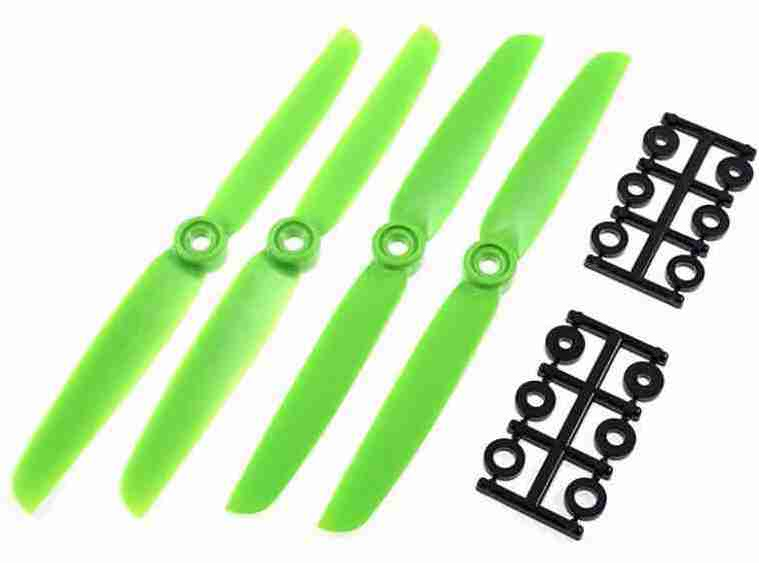
\includegraphics[width=0.45\linewidth]{fotos/helices.jpg}}

\item {\bf Cámara y transmisor de imagen. 29\euro{}.}

Enlace: \url{www.rctimer.com/product-1318.html}

Esta será la cámara y el transmisor de video que nos permitirá grabar la imagen y transmitirla a tiempo real a nuestras gafas de realidad virtual.

\centerline{
    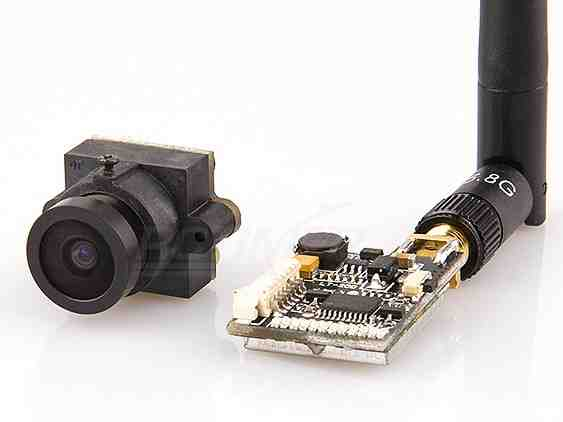
\includegraphics[width=0.45\linewidth]{fotos/camara.jpg}}


\item {\bf Módulo receptor de imagen. 28\euro{}.}

Enlace: \url{www.hobbyking.com/hobbyking/store/__83195__Fat_Shark_Raceband_5_8GHz_Module.html}

Con este módulo podemos recibir la imagen enviada por el dron para procesarla en el ordenador o mandar a las gafas de realidad aumentada del operador.

\centerline{
    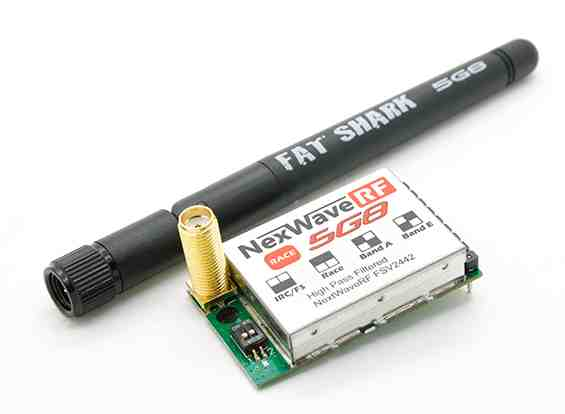
\includegraphics[width=0.45\linewidth]{fotos/receptor.jpg}}

\item {\bf Antenas de polarización circular. 20\euro{}.}

Enlace: \url{www.rctimer.com/product-1099-index.html}

Las antenas que incluyen el transmisor y el módulo receptor son de polarización lineal y nos podrían provocar problemas debido a los cambios de orientación del drone por lo que queremos comprar estas antenas de polarización circular que con un precio bastante asequible nos permitirían alcanzar más del doble de distancia si distorsiones.


\centerline{
    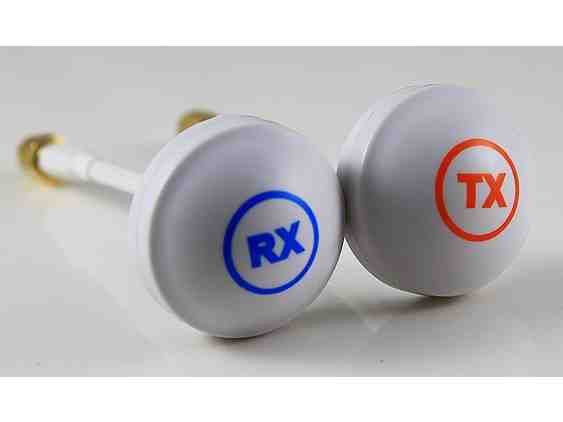
\includegraphics[width=0.45\linewidth]{fotos/antena.jpg}}

\item {\bf Gafas de realidad aumentada FPV. 320\euro{}.}

Enlace: \url{www.hobbyking.com/hobbyking/store/__84640__Fatshark_Dominator_V3_Headset_EU_Warehouse_.html}

Estas gafas son necesarias para poder pilotar el drone en primera persona (First Person View). Sabemos que son un elemento caro, pero esto nos abrirá numerosas puertas para el futuro ya que como se observa en los anteriores componentes el transmisor y la cámara son bastante baratos y podríamos realizar numerosos proyectos donde dar utilidad a estas gafas de realidad virtual. Una de las cuantiosas ventajas que tienen estas  gafas son por ejemplo unos acelerómetros que nos permitirán girar la cámara del drone (instalando dos servos) con el movimiento de nuestra cabeza, lo que daría una sensación de inmersión total.

\centerline{
    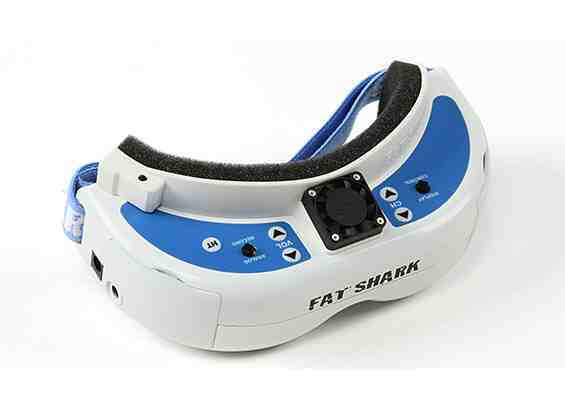
\includegraphics[width=0.45\linewidth]{fotos/gafas.jpg}}

\end{itemize}

{\bf El presupuesto total, incluyendo gastos de envio previstos, se estima en 550\euro{}.}

\subsection{Construcción Fresadora Cyclone PCB}
\subsubsection{Responsable de proyecto y equipo de trabajo}
Carlos y Victor
\subsubsection{Descripción}
\subsubsection{Objetivos}
\subsubsection{Contenido}
\subsubsection{Previsión de desarrollo}
\subsubsection{Presupuesto}


\subsection{Contrucción de un Escáner 3D}
\subsubsection{Responsable de proyecto y equipo de trabajo}
Carlos y Víctor
\subsubsection{Descripción}
Aspiramos a conseguir un Club de Robótica completamente funcional que permita a los socios realizar proyectos de robótica de una forma rápida y eficiente, para ello creemos fundamental agilizar el transito de la idea incial del proyecto a los primeros protipos funcionales y hasta la versión final del mismo. \\
Con este objetivo construimos la primera impresora 3D de la universidad. Creemos que la impresora 3D, junto a un escáner 3D y la fresadora Cyclone (que permite fresar circuitos electrónicos) son las herramientas modernas fundamentales para este proceso ágil.

\subsubsection{Objetivos}
Construcción del escáner 3D Ciclop diseñado y distribuido como kit de piezas por la empresa española BQ.\\
Además de adquirir una nueva herramiento de grandisima utilidad para el club, al ser un proyecto de construcción (ya que se compra el kit de piezas unicamente) tenemos el objetivo de aprender y profundizar en el diseño 3D, en la construcción de sistemas hardware y el software de escaneo y modelado 3D.
%\subsubsection{Contenido}

\subsubsection{Previsión de desarrollo}
La previsión de desarrollo del proyecto de montaje se estima en 2 semanas a partir del momento en el que el kit llegue al taller.\\
Con el escáner Ciclop ya montado comenzará la etápa de adaptación del software existente a los que euqipos disponibles en el taller y la fase más importante de pruebas, calibrado y puesta a punto.
\subsubsection{Presupuesto}
La empresa BQ proporciona un kit completo de piezas los que nos permite acortar la étapa de adquisición de los materiales de forma muy notable e incluso ahorrar costes al adquirirlo todo en un mismo distribuidor. \\
\\
El precio del kit es 249,90\euro{}.\\
Enlace: \url{www.bq.com/es/ciclop}

\section{Organización de talleres formativos para alumnos de la Universidad}

\subsection{Taller: Introducción a las FPGAs}
\subsubsection{Responsable de proyecto y equipo de trabajo}
Carlos
\subsubsection{Descripción}
\subsubsection{Objetivos}
\subsubsection{Contenido}
\subsubsection{Previsión de desarrollo}
\subsubsection{Presupuesto}


\subsection{Taller: Diseño e Impresión 3D (Open Hardware)}
\subsubsection{Responsable de proyecto y equipo de trabajo}
Carlos y Victor
\subsubsection{Descripción}
Se trata de un taller de modelado 3D orientado a la robótica, daremos una introducción a los participantes del uso de la herramienta libre OpenSCAD para el diseño de piezas 3D. Además queremos realizar pequeños retos prácticos en los que los participantes puedan poner en práctica lo aprendido. También se dará una charla sobre impresión 3D y finalizaremos mostrando como utilizar la impresora 3D existente en el club imprimiendo los mejores trabajos realizados por los participantes.
\subsubsection{Objetivos}
Queremos fomentar el diseño de open hardware entre los estudiantes de la universidad.

También queremos que los estudiantes aprendan utilizar la impresora 3D y sean libres de imprimir durante el curso piezas que necesiten para sus proyectos.

Por último queremos enseñar las ventajas y desventajas de imprimir con plástico o madera y cuándo puede ser útil cada uno de estos materiales

\subsubsection{Contenido}
El contenido del curso será:
\begin{itemize}
	\item Introducción teórica a OpenSCAD
	\item Retos por parejas para poner en práctica lo aprendido.
	\item Exposición de los robots que se han construido con la impresora 3D en el CRM.
	\item Diseño libre por parejas de piezas imprimibles para la construcción de un robot.
	\item Explicación del funcionamiento y manejo de la impresora 3D.
	\item Impresión de los mejores diseños que hayan hecho los estudiantes.
\end{itemize}
\centerline{
	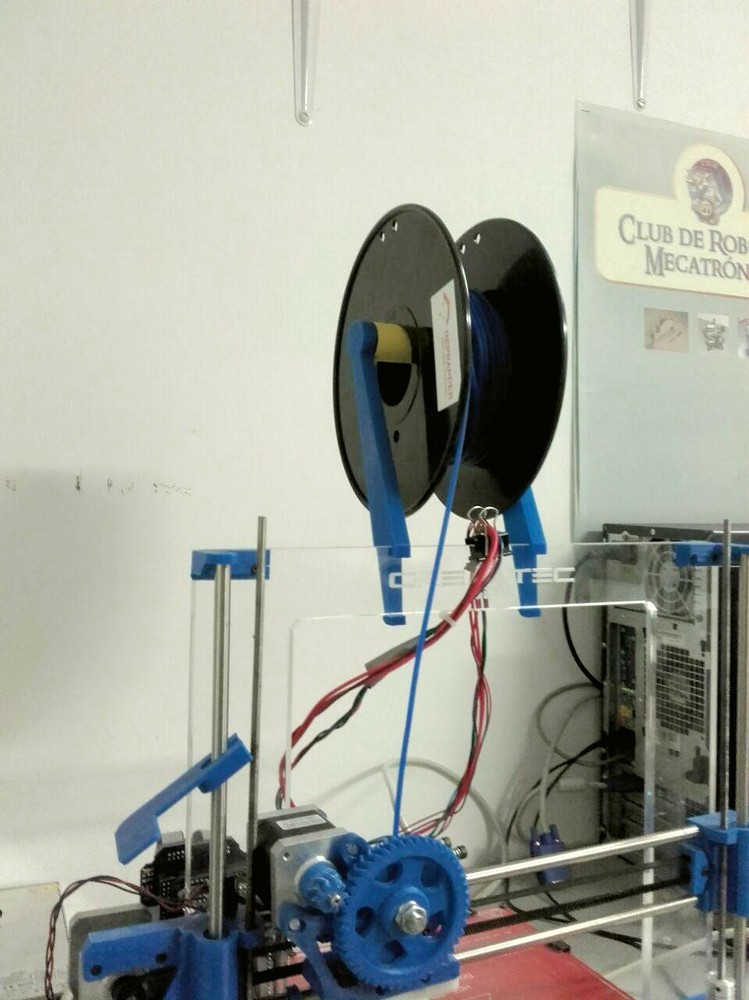
\includegraphics[width=0.3\linewidth]{fotos/photo_2015-12-14_14-01-18.jpg}
	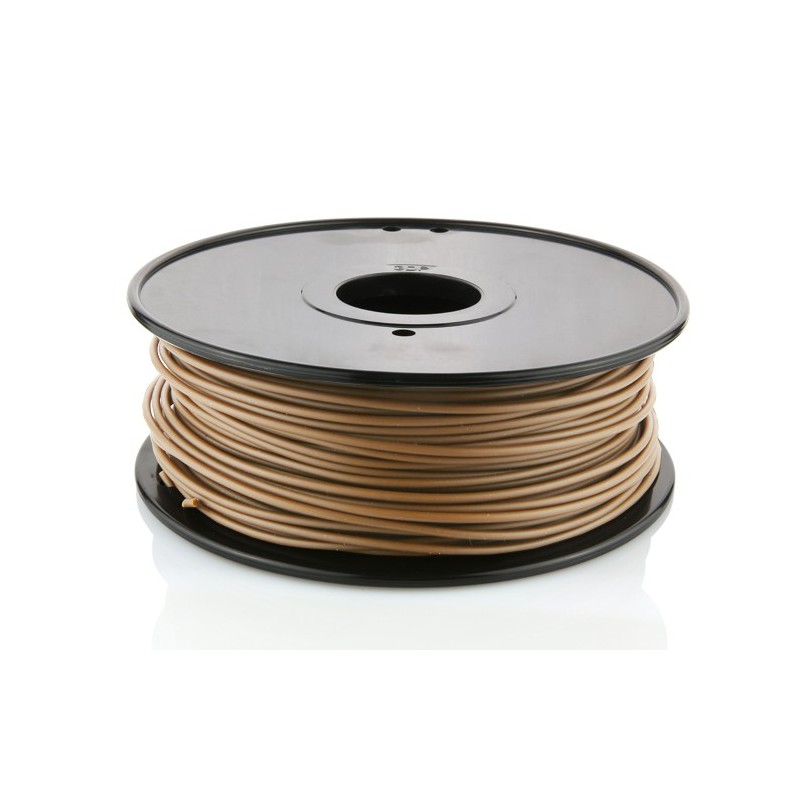
\includegraphics[width=0.3\linewidth]{fotos/filamento-madera-3mm-1kg.jpg}
	 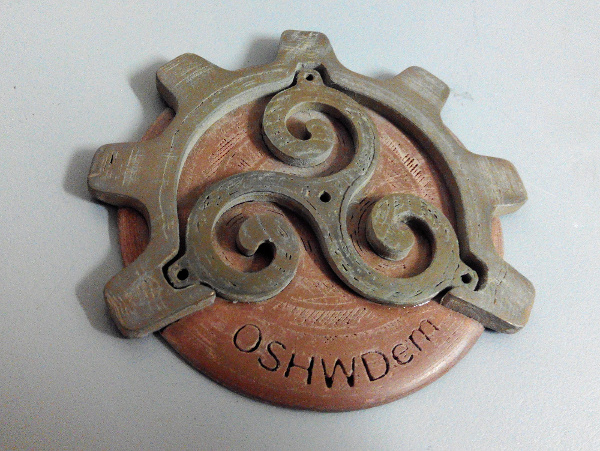
\includegraphics[width=0.3\linewidth]{fotos/trofeoOSHWDem2015.jpg}
	 }

\subsubsection{Previsión de desarrollo}
\subsubsection{Presupuesto}

\begin{table}[htbp]
	\centering\resizebox{16cm}{!} {
		\begin{tabular}{|l|l|l|l|}
			\hline
			\multicolumn{1}{|c|}{\textbf{Producto}} & \multicolumn{1}{c|}{\textbf{Encale de compra}}                                   & \multicolumn{1}{c|}{\textbf{Precio Unitario}} & \multicolumn{1}{c|}{\textbf{Unidades}} \\ \hline
			Bobina filamento de madera                   & \scalebox{.8}{\href{http://www.amazon.es/Ice-Filaments-ICEFIL3WOO182-Filamento-Madera/dp/B017HAIPVG/ref=sr_1_5?ie=UTF8&qid=1450094119&sr=8-5&keywords=filamento+madera+3d+3mm}{http://goo.gl/ghE447}}              & 31,90\euro{}                                        & 1                                      \\ \hline

			Bobina filameto de plástico                       & \scalebox{.8}{\href{http://www.amazon.es/gp/offer-listing/B00LXK7U40/ref=dp_olp_0?ie=UTF8&condition=all&qid=1450094934&sr=8-7}{http://goo.gl/6PKl8U}} & 19,90 + 6,90\euro{}                                        & 2                                      \\ \hline
			Laca impresora                       & \scalebox{.8}{\href{http://goo.gl/OEVBDj}{http://goo.gl/OEVBDj}} & 5,50\euro{}                                        & 1                                      \\ \hline
		\end{tabular}
	}
	\centering
	\caption{presupuesto taller de diseño e impresión 3d}
\end{table}



\subsection{Taller: Introducción a la robótica con Arduino}
\subsubsection{Responsable de proyecto y equipo de trabajo}
\subsubsection{Descripción}
Es habitual en el Club de Robótica realizar un taller prático de introducción a la robótica para los alumnos de la Escuela Politécnica Superior. Consideramos muy importante de cara al año que viene realizar este taller para dar a conocer el club a nuevos alumnos con interés en robótica pero sin conocimientos previos.
\begin{figure}[hbtp]
\centerline{
\includegraphics[width=0.33\linewidth]{fotos/2012_taller_arduino_pantallas.jpg} 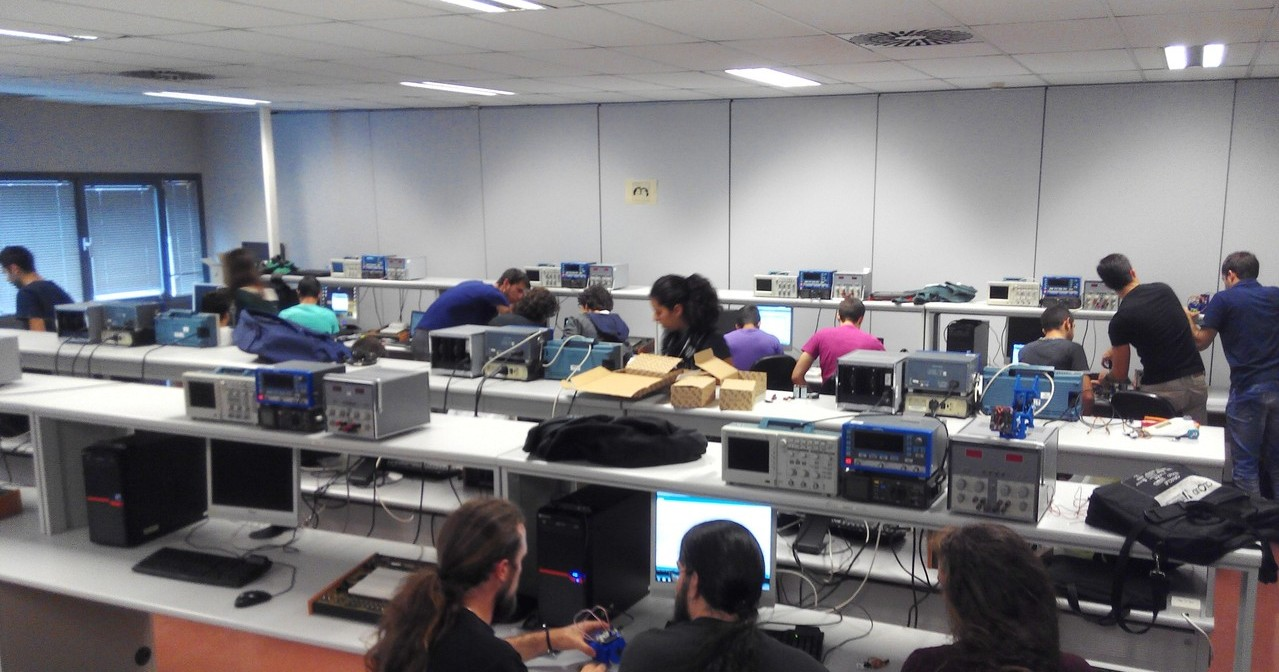
\includegraphics[width=0.4\linewidth]{fotos/fotoParticipantesArduparty.jpg} 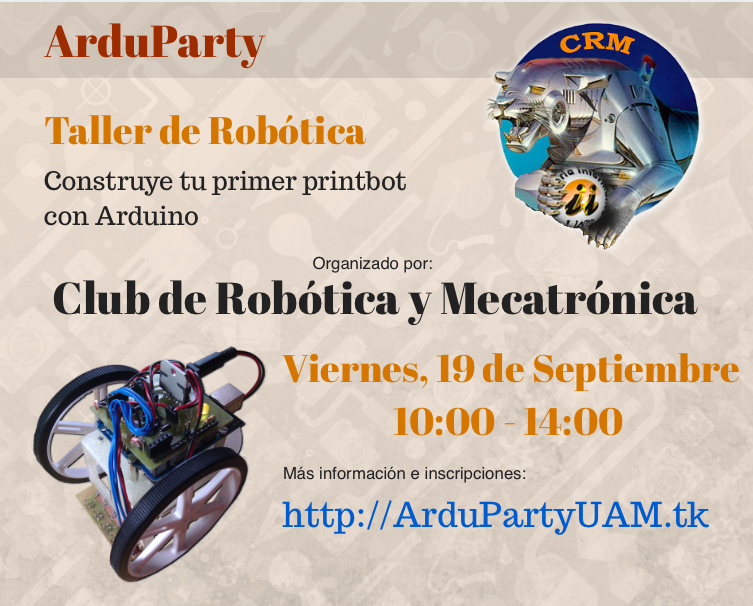
\includegraphics[width=0.33\linewidth]{fotos/2014_Cartel_ArduParty.png}}
\caption*{
Ediciones previas del taller.
}
\end{figure}

\subsubsection{Objetivos}
Seguir fomentado el conocimiento de la robótica entre los estudiantes de carreras técnicas. Dar a conocer nuestra asociación a estudiantes interesados y la nueva disponibilidad del taller del club para intenta fomentar que se creen nuevos grupos de trabajo autónomos dentro de la asociación.\\
Tenemos que seguir ofreciendo cada vez a más estudiante la posibilidad de realizar proyectos novedosos en el ámbito de la robótica y darles un pequeño empujón y respaldo necesario para llevarlos a cabo.\\
Acercar la plataforma Arduino, el diseño de Open Hardware y el diseño de estructuras 3D.
\subsubsection{Contenido}
El contenido del curso es fundamentalmente el mismo que el de la edición pasado, reutilizaremos los robots diseñados especificamente para esa edición basados en la plataforma Arduino. Los participantes tendran que realizar el montaje de sus kits y las conexiones electricas. \\
\begin{figure}[hbtp]
\centerline{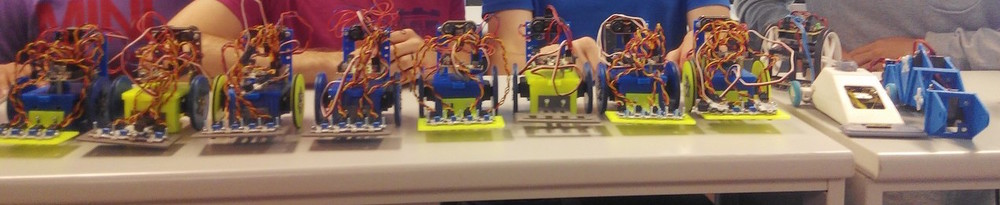
\includegraphics[width=1\linewidth]{fotos/robots_ArduParty.jpg}}
\caption*{
Robots ensamblados.
}
\end{figure}
Con el robot ya montado realizarmos diversas prácticas de programación y realizaremos interesantes retos guiando a los participantes en todo momento e introduciendoles de esta forma en la plataforma Arduino.\\
También profundizaremos en la comunicación entre Android y Arduino (Smartphone y Robot) programando una aplicación sencilla que nos permita controlar el robot desde el móvil.
\subsubsection{Previsión de desarrollo}
\subsubsection{Presupuesto}
Reutilizaremos los robots montados en la pasada edición del taller por lo que el presupuesto necesario es mínimo. \\
Para mejorar y suplir las deficiencias de la pasada edición necesitamos comprar baterías (pilas recargables) y cargadores para tener una mayor autonomía.\\
\begin{table}[htbp]
\centering\resizebox{16cm}{!} {
\begin{tabular}{|l|l|l|l|}
\hline
\multicolumn{1}{|c|}{\textbf{Producto}} & \multicolumn{1}{c|}{\textbf{Encale de compra}}                                   & \multicolumn{1}{c|}{\textbf{Precio Unitario}} & \multicolumn{1}{c|}{\textbf{Unidades}} \\ \hline
Pilas Recargables 9V                    & \scalebox{.8}{\href{http://es.rs-online.com/web/p/pilas-recargables-9-voltios/7033524/}{es.rs-online.com/web/p/pilas-recargables-9-voltios/7033524/}}              & 10,28\euro{}                                        & 8                                      \\ \hline
Cargador Pilas 9V                       & \scalebox{.8}{\href{http://es.rs-online.com/web/p/cargadores-de-pilas-aaa-aa-c-d-9- voltios/5177789/}{es.rs-online.com/web/p/cargadores-de-pilas-aaa-aa-c-d-9- voltios/5177789/}} & 15,10\euro{}                                        & 2                                      \\ \hline
\end{tabular}
}
\centering
\caption{presupuesto taller de introducción a la robótica}
\end{table}


\subsection{Taller: Sistemas embebidos. Raspberry Pi}
\subsubsection{Responsable de proyecto y equipo de trabajo}
\subsubsection{Descripción}
\subsubsection{Objetivos}
\subsubsection{Contenido}
\subsubsection{Previsión de desarrollo}
\subsubsection{Presupuesto}


\section{Organización de concursos internos y fomento de la robótica entre los estudiantes}


\section{Participación en eventos nacionales y representación de la UAM}

\section{Solicitud de subvención}




\chapter{Memoria del curso anterior}

\section{Talleres y proyectos internos}

\subsection{Re-organización del local para fomentar la participación}

\begin{itemize}
\item Actualización de la página web y creación de repositorio GitHub para el control de versiones
\item Limpieza del local (reciclado de equipos obsoletos que ocupaban espacio, mesas despejadas para facilitar la labor del equipo de limpieza)
\item Organización del material de los armarios y de las herramientas gracias a un panel de madera con ganchos.
\item Cada estudiante puede solicitar una caja de proyecto donde guardar todo el material que necesite. Dichas cajas están etiquetadas con su nombre y año, de este modo es posible organizar mejor el inventario disponible.
\end{itemize}

El nuevo enfoque del Club de Robótica es apoyar a cualquier miembro de la comunidad universitaria que quiera llevar a cabo proyectos relacionados con la robótica. Es decir, tanto estudiantes como profesores pueden inscribirse y así disponer de un espacio de trabajo agradable con herramientas de uso común (impresoras 3D, soldadores, sierras, alicates, destornilladores, etc) así como los materiales necesarios (cables, componentes, motores, baterías, etc).

Además disponemos de un foro donde nos ayudamos unos a otros, y periódicamente seguimos organizando actividades para fomentar la robótica entre los estudiantes.

\subsection{Construcción de un cuadricóptero}
\subsubsection{Participantes}

\begin{itemize}


\item Carlos García
\item Cristina Kasner
\item Jaime Aragón
\item Rodrigo Jimenez
\item Víctor Uceda
\end{itemize}

Durante el segundo cuatrimestre del curso 2014-15 hemos realizado la compra de materiales, diseño y montaje de un cuadricóptero tal como detallamos en los presupuestos del año pasado.

Durante los meses de febrero y abril realizamos las compras de los materiales presupuestados, en las que nos encontramos con agunas dificultades en los trámites aduaneros que alargó el proceso en tiempo y dinero.

Cuando conseguimos tener todas las piezas en el taller realizamos el montaje, utilizamos una configuración extandar para cuadricópteros ( en H ).

Con el cuadricoptero ya montado programamos y lo configuramos para el vuelo basandonos en firmware abierto \begin{em}multiWii\end{em}.

Una de las tareas más costosas en tiempo y delicadas fue, a partir de la construcción completa, el ajuste preciso de los parametros de vuelo para conseguir gran estabilidad sin perder el balance con la agilidad.

\begin{figure}[hbtp]
\centerline{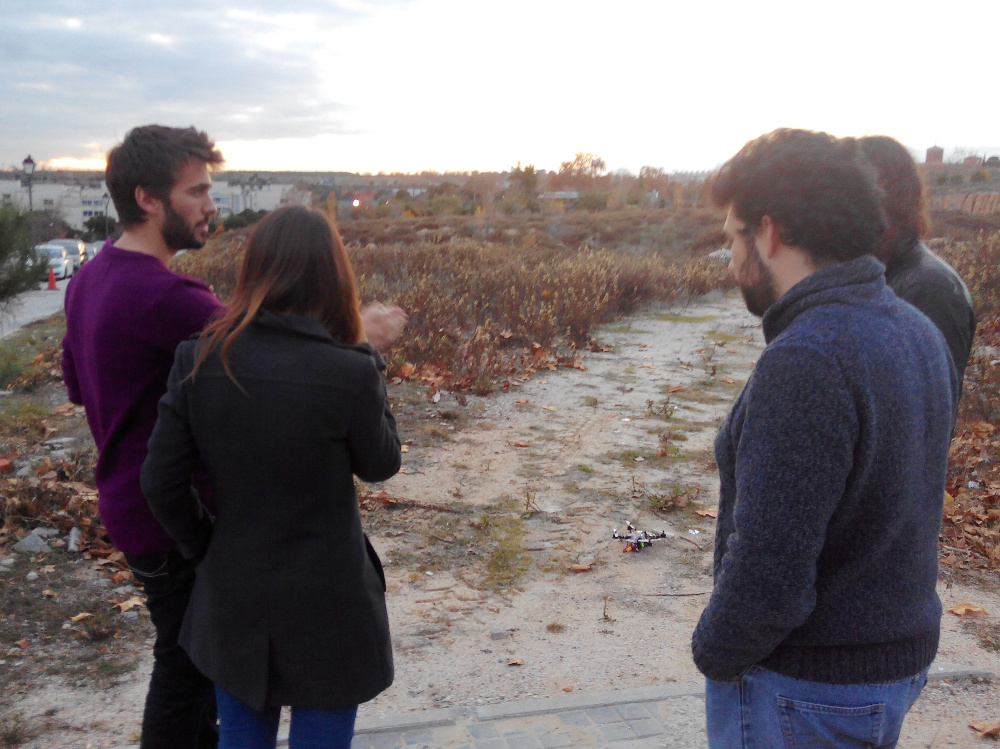
\includegraphics[width=0.4\linewidth]{fotos/2015-12-11_PruebaVuelo_JaimeCrisPabloRafa.jpg} 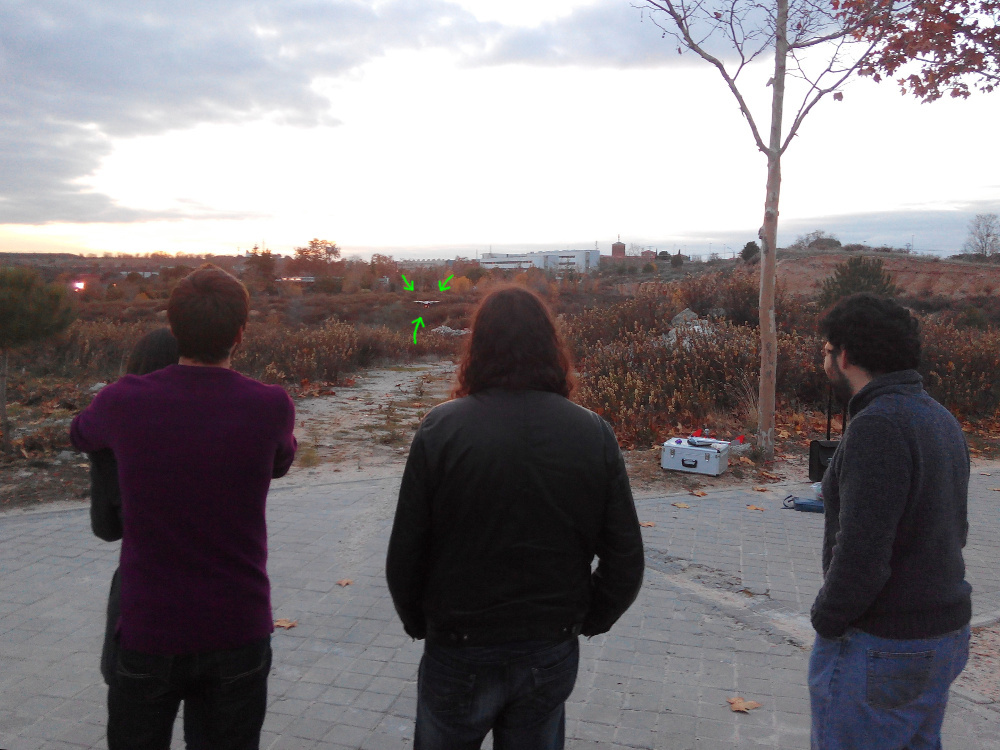
\includegraphics[width=0.4\linewidth]{fotos/2015-12-11_PruebaVuelo_CrisJaimeRafaPablo.jpg}}
\caption*{
Robots ensamblados.
}
\end{figure}

\subsection{Construcción de un robot para resolver laberintos}





\subsection{Uso de la impresora 3D por la comunidad universitaria(por estudiantes)}
Desde el Club de Robótica intentamos fomentar el uso de la impresora 3D que construimos en 2014 para todos los miembros de la comunidad universitaria.
Además de la valiosa labor que la realiza la impresora para el Club (ya que tanto los robots diseñados para los talleres, como los proyectos ya detallados usan estructuras impresas 3D) durante este año (y pese a la desorganización del taller previa a la reestructuración realizada) la impresora ha servido a multiples alumnos y personal investigador para realizar prototipos de proyectos individuales.

\begin{figure}[hbtp]
\centerline{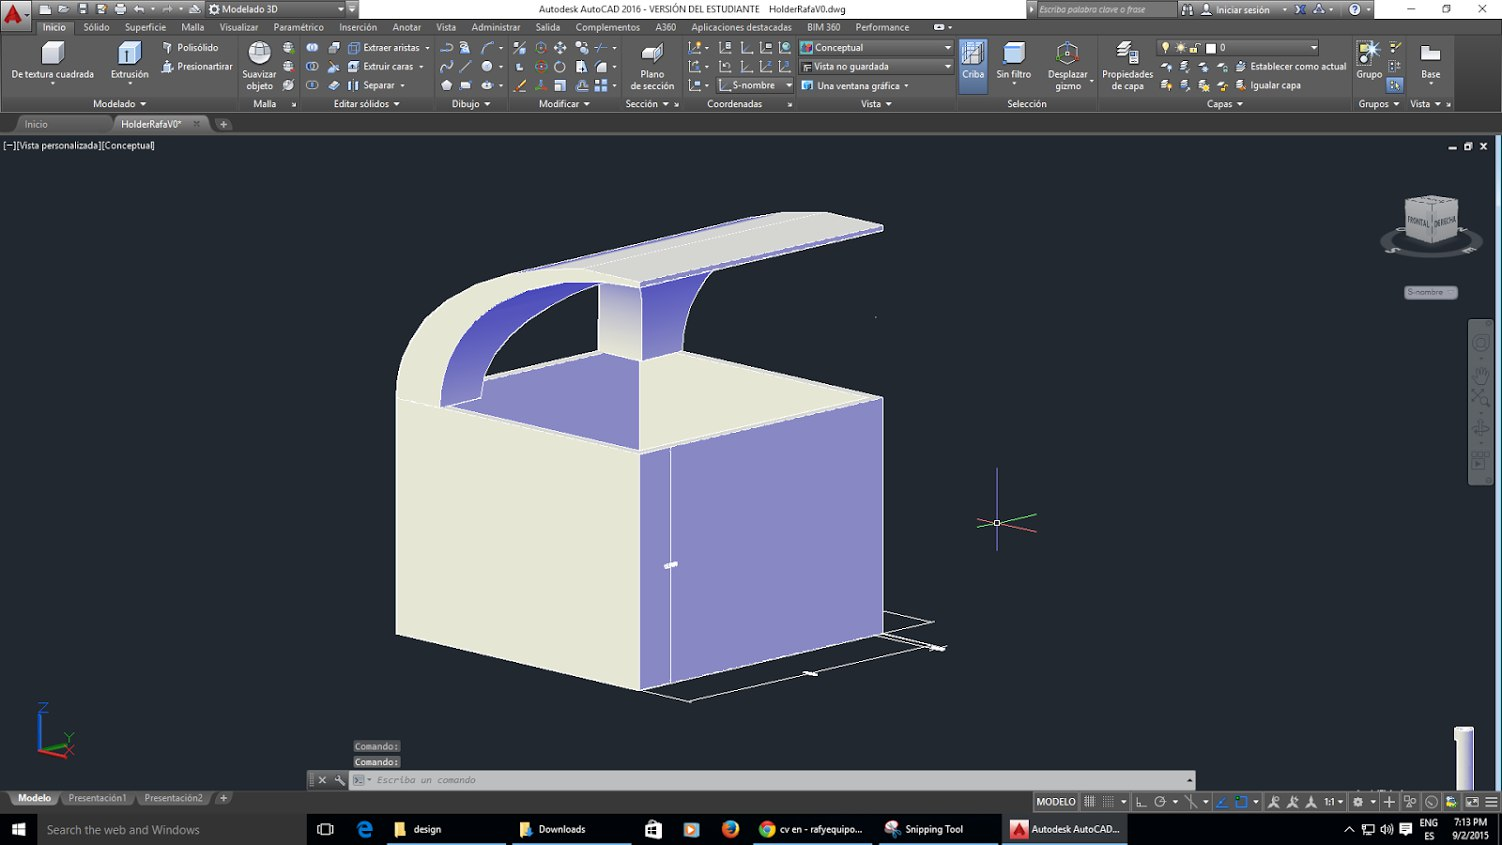
\includegraphics[width=0.3\linewidth]{fotos/impresora1.jpg} 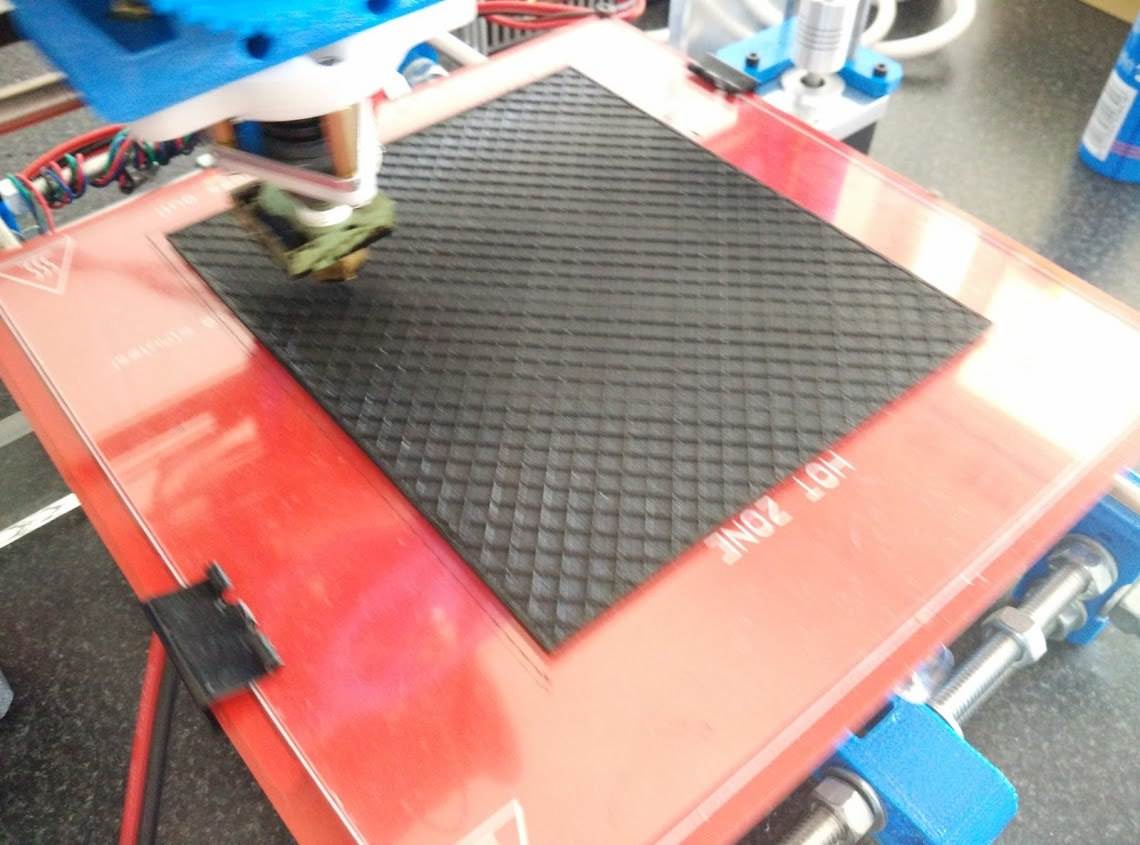
\includegraphics[width=0.3\linewidth]{fotos/impresora2.jpg} 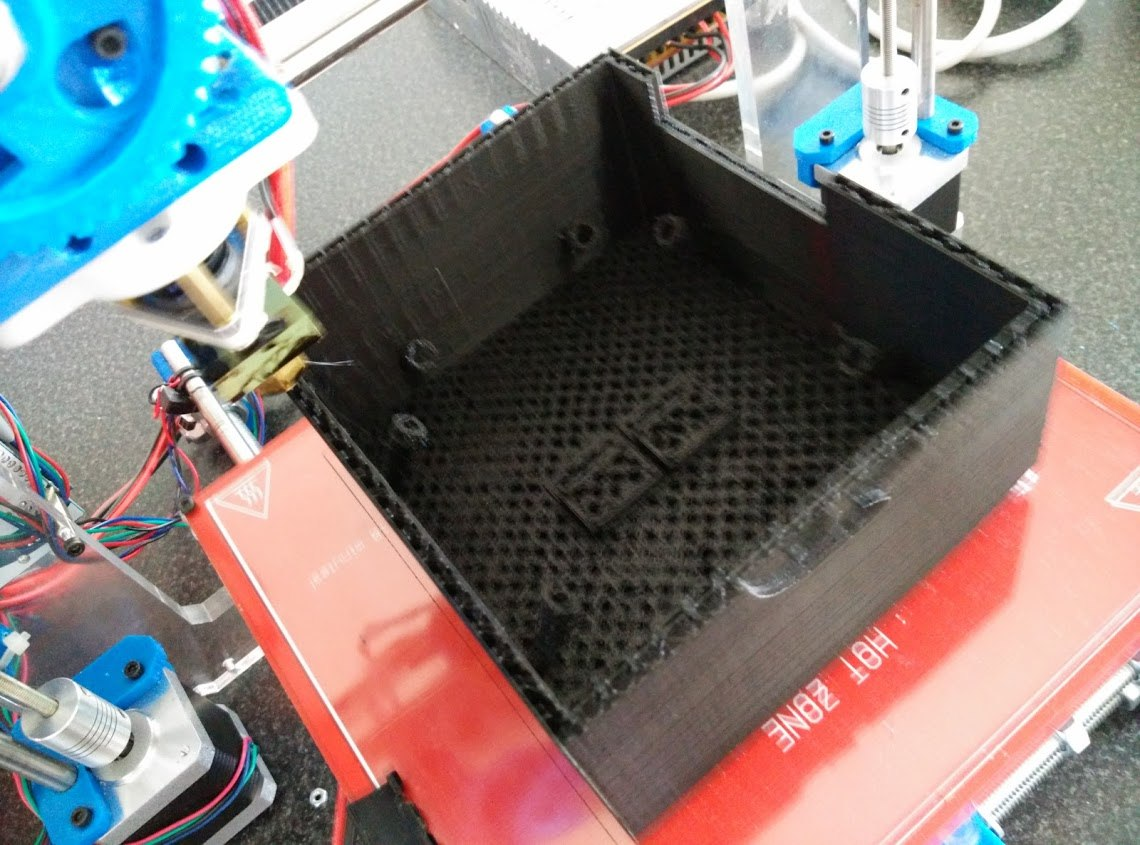
\includegraphics[width=0.3\linewidth]{fotos/impresora3.jpg}}
\centerline{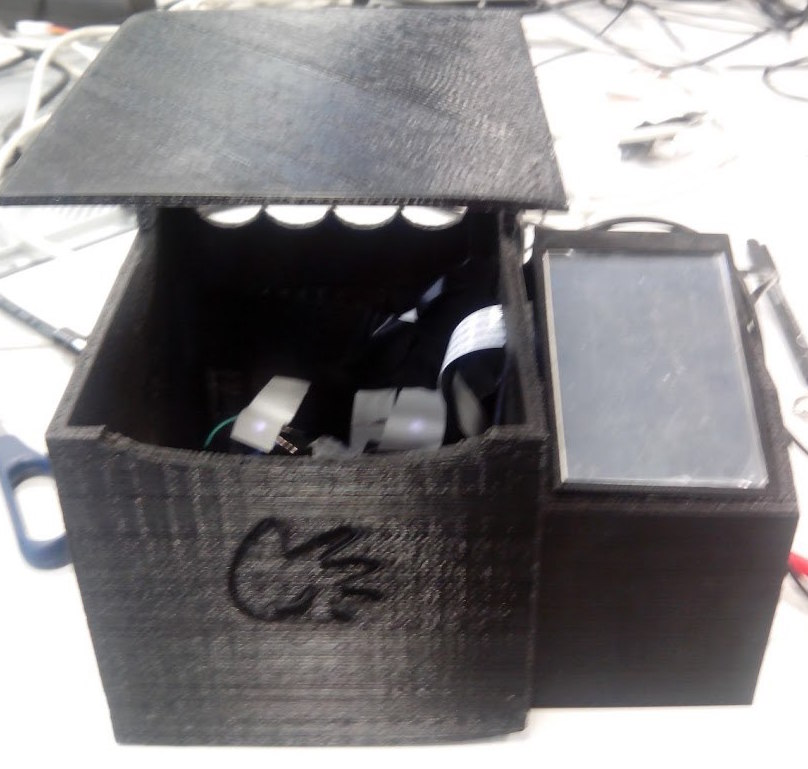
\includegraphics[width=0.4\linewidth]{fotos/impresora4.jpg}}
\caption*{
Proceso completo de impresión 3D.
}
\end{figure}

Creemos que el disponer de herramientas como esta otorgo una gran libertad a los estudiantes para lanzarse a realizar proyectos propios que pueden llegar a alcanzar un gran éxito.

\newpage

\section{Participación en eventos nacionales}


\subsection{Concurso de resolución de laberintos en la OSHWDem (Galicia, A Coruña)}

La OSHWDem (Open Source Hardware Demonstration) es un evento que se realiza anualmente en A Coruña. Allí se reúnen multitud de frikis de diversas disciplinas, y entre otras cosas se organizan competiciones de robótica\footnote{\url{http://oshwdem.org/concursos/}}.

\vspace{5mm}

\centerline{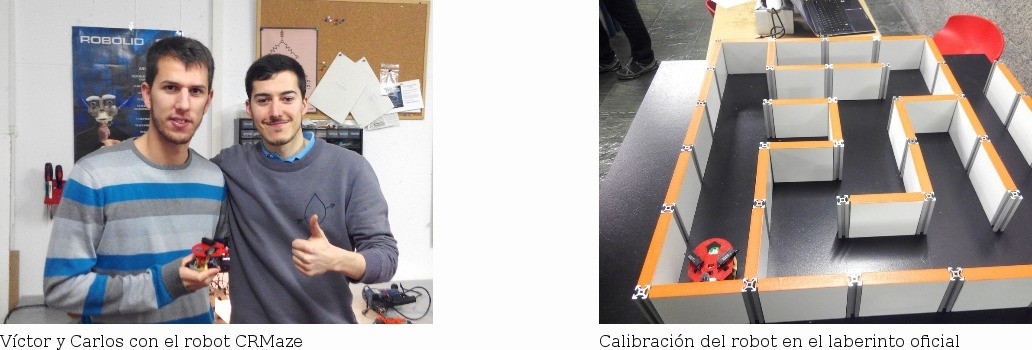
\includegraphics[width=1.1\linewidth]{fotos/oshwdem2015_robot}}

Éste año nos propusimos el reto de presentar un robot al concurso de resolución de laberintos (también conocido como \emph{micromouse}). Fue todo un reto porque tan sólo tuvimos dos semanas para construir el robot y programar los algoritmos necesarios.
El resultado fue el robot CRMaze\footnote{\url{https://github.com/CRM-UAM/CRMaze}}.


\vspace{5mm}
\centerline{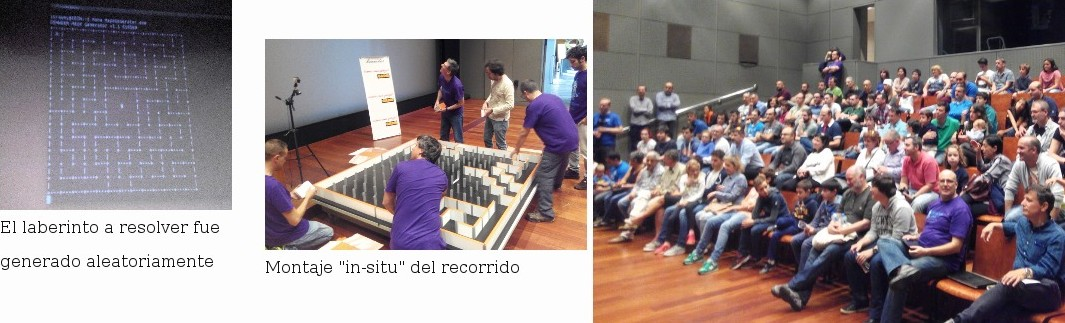
\includegraphics[width=1.1\linewidth]{fotos/oshwdem2015_laberinto}}


Aunque ninguno de los participantes fue capaz de resolver el laberinto debido a su alta complejidad, fue muy divertido y todos aprendimos mucho. Además nos dieron un trofeo impreso en 3D con filamentos de cobre y bronce.


\begin{wrapfigure}[10]{l}{7cm}\centering
    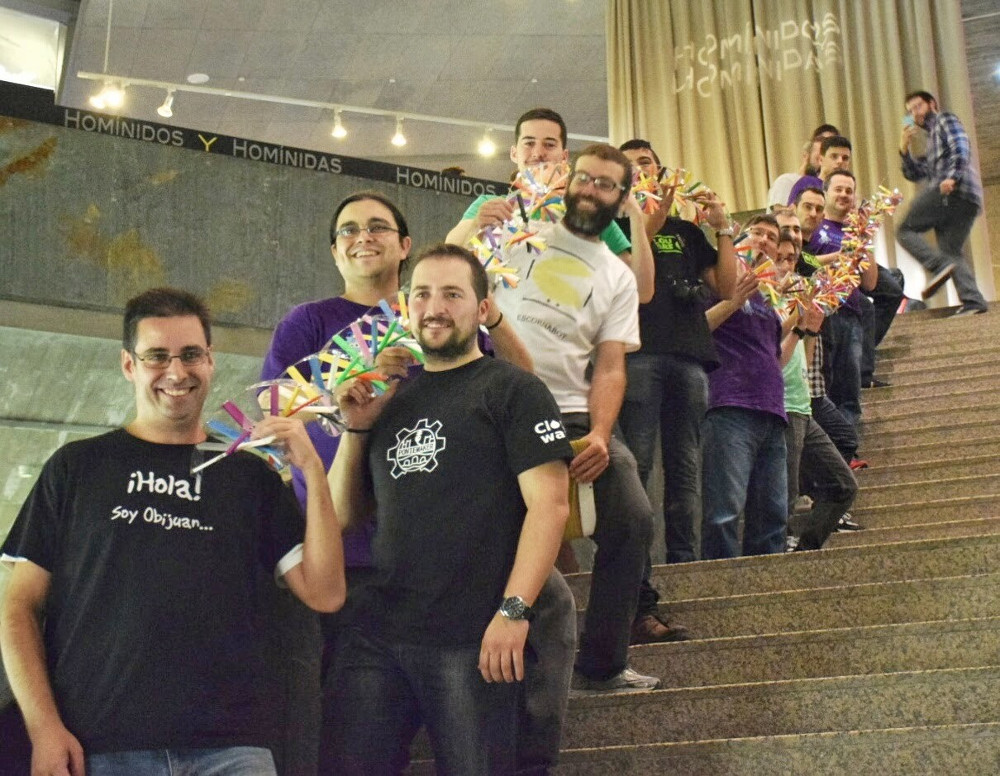
\includegraphics[scale=0.2]{fotos/2015_OSHWDem_cadenaADNcloneWars}
    \caption*{}
\end{wrapfigure}
También participamos en el reto \emph{ADN CloneWars}\footnote{\url{https://github.com/brico-labs/RetoADNCloneWars}}. En él se imprimieron más de 500 piezas para construir una cadena de ADN con los nombres de todas las impresoras open-source construidas en España dentro del grupo RepRap Clone Wars\footnote{\url{www.reprap.org/wiki/Clone_wars}}.

El Club de Robótica forma una parte importante de la cadena ya que el clon Nº5, \emph{Halcón Milenario}, fue construido en 2012 en el local de la asociación.

Para el año que viene nos hemos propuesto mejorar el diseño del CRMaze para conseguir resolver el laberinto por fin, y además queremos crear equipos que participen en otros concursos dentro de la OSHWDem (seguidores de línea, robots de sumo y de combate).



\subsection{Asistencia a la V jornada GMV de robótica (Madrid, Tres Cantos)}


El 26 de Noviembre de 2015 asistimos desde el Club de Robótica al evento que tuvo lugar en la sede oficial de GMV, situada en Tres Cantos. Allí se realizaron demostraciones en directo de los robots Foxiris (para monitorización de plantas oil \& gas), MiR100 (un robot de exploración de tipo rover) y Aunav (un robot usado para la desactivación de explosivos)\footnote{\tiny\url{http://www.gmv.com/es/Empresa/Comunicacion/NotasDePrensa/2015/NP_017_VJornadaRobotica.html}}.

\begin{figure}[hbtp]
\centerline{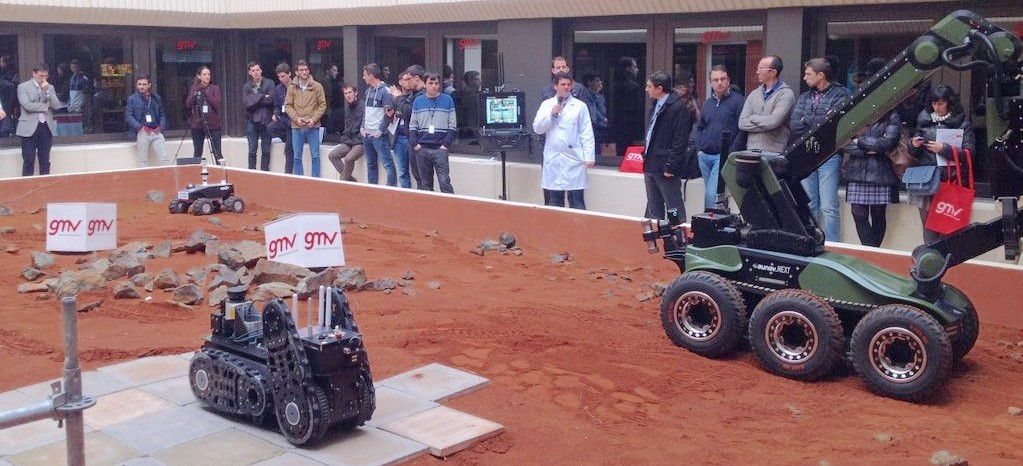
\includegraphics[width=0.8\linewidth]{fotos/2015_V_JornadaRobotica_GMV}}
\caption*{
Demostración de los robots Foxiris de GMV (izquierda), MiR100 de Robotplus (al fondo) y Aunav de Proytecsa (derecha).
}
\end{figure}

Además participamos en el concurso ``Concurrent Design Facility (CDF) for Robotics'' en el que se nos asignó la tarea de diseñar un robot para la monitorización de plantas oil \& gas en menos de tres horas. Obtuvimos el primer premio junto con estudiantes de la UPM.


\begin{figure}[hbtp]
\centerline{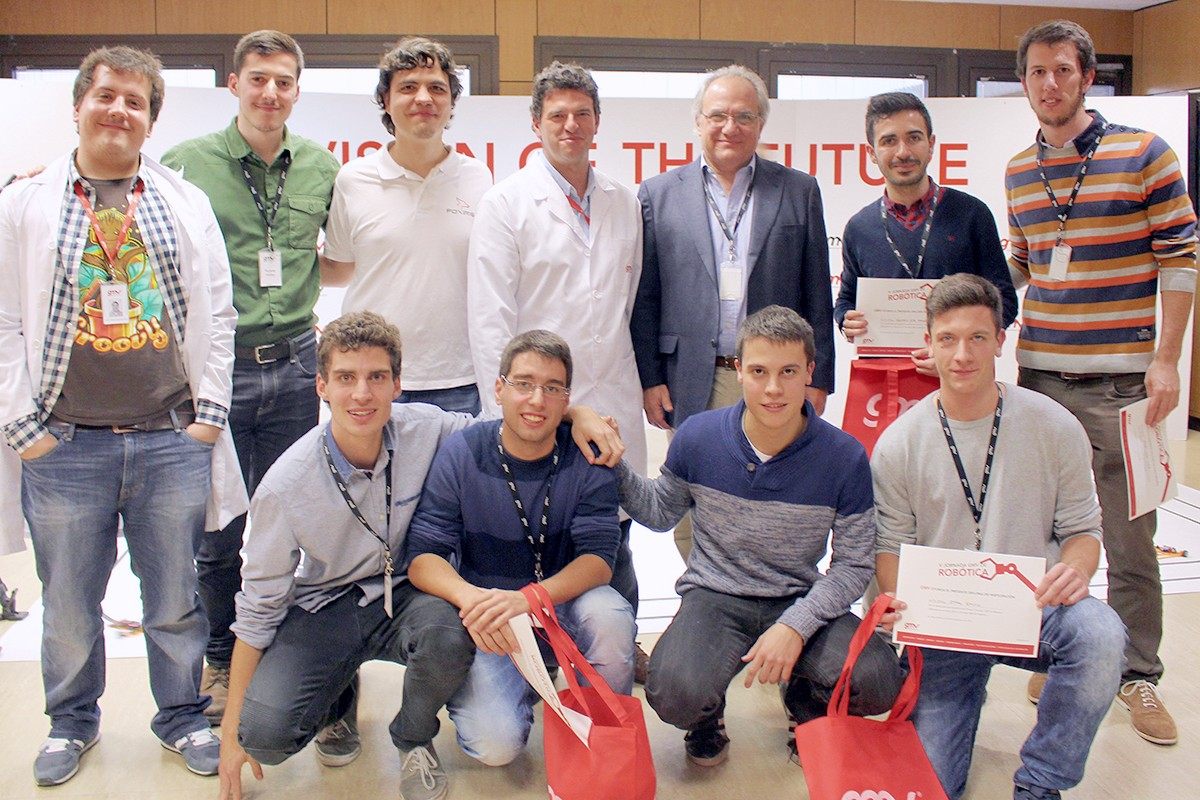
\includegraphics[width=0.8\linewidth]{fotos/2015_V_JornadaRobotica_GMV_team}}
\caption*{
Participantes en el concurso ``Concurrent Design Facility (CDF) for Robotics''. \\
Fila superior: Carlos Crespo (GMV), Carlos García (CRM-UAM), Sergio Martini (GMV), Alberto Medina (GMV), Pedro Hernández (Repsol), Gonzalo Díaz (UPM) y Víctor Uceda (CRM-UAM)
Fila inferior: Luis Paarup, David Matilla, Javier Fernández, Stefan y Pablo Rodríguez -ausente en la foto- (todos de la UPM)
}
\end{figure}






\chapter{Junta directiva actualizada}

La Asociación Club de Robótica-Mecatrónica cuenta con la siguiente junta directiva para el curso 2015-16:

\begin{itemize}
\item Presidente: \textbf{Carlos García Saura} (carlos.garciasaura*)
\item Vice-presidente: \textbf{Rodrigo José Jiménez} (rodrigojose.jimenez*)
\item Secretario: \textbf{Cristina Kasner Tourné} (cristina.kasner*)
\item Tesorero: \textbf{Jaime Eduardo Aragón} (jaimeeduardo.aragon*)
\item Vocales: \textbf{Víctor Uceda Uceda} (vic.uceda*) y \textbf{Pablo Molins Ruano} (pablo.molins*)
\end{itemize}

* \textit{correos electrónicos a completar con ``@estudiante.uam.es''}

En la página web de la asociación está disponible toda la información sobre la organización del club en años anteriores:
\url{http://crm.ii.uam.es/historia}


\end{document}
